%% BioMed_Central_Tex_Template_v1.06
%%                                      %
%  bmc_article.tex            ver: 1.06 %
%                                       %

%%IMPORTANT: do not delete the first line of this template
%%It must be present to enable the BMC Submission system to
%%recognise this template!!

%%%%%%%%%%%%%%%%%%%%%%%%%%%%%%%%%%%%%%%%%
%%                                     %%
%%  LaTeX template for BioMed Central  %%
%%     journal article submissions     %%
%%                                     %%
%%          <8 June 2012>              %%
%%                                     %%
%%                                     %%
%%%%%%%%%%%%%%%%%%%%%%%%%%%%%%%%%%%%%%%%%


%%%%%%%%%%%%%%%%%%%%%%%%%%%%%%%%%%%%%%%%%%%%%%%%%%%%%%%%%%%%%%%%%%%%%
%%                                                                 %%
%% For instructions on how to fill out this Tex template           %%
%% document please refer to Readme.html and the instructions for   %%
%% authors page on the biomed central website                      %%
%% http://www.biomedcentral.com/info/authors/                      %%
%%                                                                 %%
%% Please do not use \input{...} to include other tex files.       %%
%% Submit your LaTeX manuscript as one .tex document.              %%
%%                                                                 %%
%% All additional figures and files should be attached             %%
%% separately and not embedded in the \TeX\ document itself.       %%
%%                                                                 %%
%% BioMed Central currently use the MikTex distribution of         %%
%% TeX for Windows) of TeX and LaTeX.  This is available from      %%
%% http://www.miktex.org                                           %%
%%                                                                 %%
%%%%%%%%%%%%%%%%%%%%%%%%%%%%%%%%%%%%%%%%%%%%%%%%%%%%%%%%%%%%%%%%%%%%%

%%% additional documentclass options:
%  [doublespacing]
%  [linenumbers]   - put the line numbers on margins

%%% loading packages, author definitions

%\documentclass[twocolumn]{bmcart}
% uncomment this for twocolumn layout and comment line below
\documentclass{bmcart}

%%% Load packages
%\usepackage{amsthm,amsmath}
%\RequirePackage{natbib}
\RequirePackage{hyperref}
% \usepackage{etoolbox}
\usepackage[utf8x]{inputenc} %unicode support
\usepackage{graphicx}
\usepackage{tikz}
\usepackage{amsmath}
\usepackage{listings}
\usepackage{bera}
\usepackage{multirow}
\usepackage{fancyvrb}
\usepackage{soul}
%\usepackage[applemac]{inputenc} %applemac support if unicode package fails
%\usepackage[latin1]{inputenc} %UNIX support if unicode package fails

%%%%%%%%%%%%%%%%%%%%%%%%%%%%%%%%%%%%%%%%%%%%%%%%%
%%                                             %%
%%  If you wish to display your graphics for   %%
%%  your own use using includegraphic or       %%
%%  includegraphics, then comment out the      %%
%%  following two lines of code.               %%
%%  NB: These line *must* be included when     %%
%%  submitting to BMC.                         %%
%%  All figure files must be submitted as      %%
%%  separate graphics through the BMC          %%
%%  submission process, not included in the    %%
%%  submitted article.                         %%
%%                                             %%
%%%%%%%%%%%%%%%%%%%%%%%%%%%%%%%%%%%%%%%%%%%%%%%%%

%\def\includegraphic{}
%\def\includegraphics{}
\errorcontextlines 10000

% \makeatletter
% \patchcmd{\@addmarginpar}{\ifodd\c@page}{\ifodd\c@page\@tempcnta\m@ne}{}{}
% \makeatother
% \reversemarginpar

%%% Put your definitions there:
\startlocaldefs
  \newcommand{\comment}[2]{\hspace{0in}#2}
  \lstdefinelanguage{json}{
      basicstyle=\normalfont\ttfamily,
      numbersep=8pt,
      showstringspaces=false,
      breaklines=true,
      frame=lines,
      backgroundcolor=\color{white},
  }
\endlocaldefs


%%% Begin ...
\begin{document}

%%% Start of article front matter
\begin{frontmatter}

\begin{fmbox}
\dochead{Software}

%%%%%%%%%%%%%%%%%%%%%%%%%%%%%%%%%%%%%%%%%%%%%%
%%                                          %%
%% Enter the title of your article here     %%
%%                                          %%
%%%%%%%%%%%%%%%%%%%%%%%%%%%%%%%%%%%%%%%%%%%%%%

\title{``gnparser'':  A powerful semantic parser for scientific names based on
  parsing expression grammars}


%%%%%%%%%%%%%%%%%%%%%%%%%%%%%%%%%%%%%%%%%%%%%%
%%                                          %%
%% Enter the authors here                   %%
%%                                          %%
%% Specify information, if available,       %%
%% in the form:                             %%
%%   <key>={<id1>,<id2>}                    %%
%%   <key>=                                 %%
%% Comment or delete the keys which are     %%
%% not used. Repeat \author command as much %%
%% as required.                             %%
%%                                          %%
%%%%%%%%%%%%%%%%%%%%%%%%%%%%%%%%%%%%%%%%%%%%%%

\author[
   addressref={aff1},
   corref={aff1},                       % id of corresponding address, if any
   email={mozzheri@illinois.edu}
]{\inits{DYM}\fnm{Dmitry Y.} \snm{Mozzherin}}
\author[                  % id's of addresses, e.g. {aff1,aff2}
   addressref={aff2},
   noteref={n1},% id's of article notes, if any
   email={alexander@myltsev.com}   % email address
]{\inits{AAM}\fnm{Alexander A.} \snm{Myltsev}}
\author[
   addressref={aff3},
   email={dpatterson.mbl@gmail.com}
]{\inits{DJP}\fnm{David J.} \snm{Patterson}}

%%%%%%%%%%%%%%%%%%%%%%%%%%%%%%%%%%%%%%%%%%%%%%
%%                                          %%
%% Enter the authors' addresses here        %%
%%                                          %%
%% Repeat \address commands as much as      %%
%% required.                                %%
%%                                          %%
%%%%%%%%%%%%%%%%%%%%%%%%%%%%%%%%%%%%%%%%%%%%%%

\address[id=aff1]{                     % unique id
  \orgname{University of Illinois},    % university, etc
  \street{1816 South Oak St.},         %
  \city{Champaign},                    % city
  \state{IL},
  \postcode{61820},
  \cny{US}                             % country
}

\address[id=aff2]{                     % unique id
  \orgname{IP Myltsev},                % university, etc
  \street{Kaslinskaya St.},            %
  \city{Chelyabinsk},                  % city
  \state{},
  \postcode{454084},
  \cny{Russia}                         % country
}

\address[id=aff3]{                     % unique id
  \orgname{University of Sydney},      % university, etc
  \city{Sydney},                       % city
  \cny{Australia}                      % country
}

%%%%%%%%%%%%%%%%%%%%%%%%%%%%%%%%%%%%%%%%%%%%%%
%%                                          %%
%% Enter short notes here                   %%
%%                                          %%
%% Short notes will be after addresses      %%
%% on first page.                           %%
%%                                          %%
%%%%%%%%%%%%%%%%%%%%%%%%%%%%%%%%%%%%%%%%%%%%%%

\begin{artnotes}
%\note{Sample of title note}     % note to the article
\note[id=n1]{Equal contributor} % note, connected to author
\end{artnotes}

\end{fmbox}% comment this for two column layout

%%%%%%%%%%%%%%%%%%%%%%%%%%%%%%%%%%%%%%%%%%%%%%
%%                                          %%
%% The Abstract begins here                 %%
%%                                          %%
%% Please refer to the Instructions for     %%
%% authors on http://www.biomedcentral.com  %%
%% and include the section headings         %%
%% accordingly for your article type.       %%
%%                                          %%
%%%%%%%%%%%%%%%%%%%%%%%%%%%%%%%%%%%%%%%%%%%%%%

\begin{abstractbox}

\begin{abstract} % abstract

  \parttitle{Background} We will be able to investigate biology in new and
  different ways and on grander scales when we can integrate biological data
  from multiple sources. An obvious contribution to this vision lies in the use of scientific names
  of organisms as metadata which can bring together different pieces of information on the same taxa but which are currently held in many different places. There are impediments to transforming the concept into robust and reliable infrastructure because there is often more than one name for a taxon, or one name may apply to different taxa.  Names are
  represented by a combination of characters, spaces and
  punctuation that we refer to as a name-string'. The same names may be
  represented by many different name-strings in which elements are spelled differently, abbreviated, annotated, or include or exclude
  authors of names and dates of establishment. We can minimize mismatches
  caused by such differences if we divide the name-strings into their component
  elements and establish the roles of each element. This process is 'semantic
  parsing'. Once done, we can improve the matching of different name-strings for the same species by, for example, relying on the most widely used elements
  of names and/or by setting aside elements that differ or are rare.

  \parttitle{Results} We introduce Global Names Parser (\textit{gnparser}), a Java tool written in Scala language (a language for Java Virtual Machine) to parse scientific names that is based on a Parsing Expression Grammar. The parser can be applied to scientific name-strings of any complexity. It assigns a semantic meaning
  (such as genus name, species epithet, annotation, rank, year of publication,
  names of authors, annotations, etc.) to all elements of a name-string. It is able to work with nested structures within certain types of name-string such as the name of hybrids, and can combine more atomic elements into larger semantically meaningful elements. \textit{gnparser} performs with $\approx
  99\%$ accuracy and processes 21.4 million name-strings/hour per CPU. The \textit{gnparser} library is compatible
  with Scala, Java, R, Jython, and JRuby. The parser can be used as a command
  line application, as a socket server, a web-app or as a RESTful http-service. It is
  released under an Open Source MIT license.

  \parttitle{Conclusions} Global Names Parser (\textit{gnparser}) is a fast,
  high precision tool for bioinformaticians and biologists working with large
  numbers of scientific names. It can replace expensive and error-prone manual
  parsing and standardization of scientific names in many situations and
  can quickly enhance the interoperability of distributed biological information.

\end{abstract}

%%%%%%%%%%%%%%%%%%%%%%%%%%%%%%%%%%%%%%%%%%%%%%
%%                                          %%
%% The keywords begin here                  %%
%%                                          %%
%% Put each keyword in separate \kwd{}.     %%
%%                                          %%
%%%%%%%%%%%%%%%%%%%%%%%%%%%%%%%%%%%%%%%%%%%%%%

\begin{keyword}
\kwd{biodiversity}
\kwd{biodiversity informatics}
\kwd{scientific name}
\kwd{parser}
\kwd{semantic parser}
\kwd{names-based cyberinfrastructure}
\end{keyword}

% MSC classifications codes, if any
%\begin{keyword}[class=AMS]
%\kwd[Primary ]{}
%\kwd{}
%\kwd[; secondary ]{}
%\end{keyword}

\end{abstractbox}
%
%\end{fmbox}% uncomment this for twcolumn layout

\end{frontmatter}

%%%%%%%%%%%%%%%%%%%%%%%%%%%%%%%%%%%%%%%%%%%%%%
%%                                          %%
%% The Main Body begins here                %%
%%                                          %%
%% Please refer to the instructions for     %%
%% authors on:                              %%
%% http://www.biomedcentral.com/info/authors%%
%% and include the section headings         %%
%% accordingly for your article type.       %%
%%                                          %%
%% See the Results and Discussion section   %%
%% for details on how to create sub-sections%%
%%                                          %%
%% use \cite{...} to cite references        %%
%%  \cite{koon} and                         %%
%%  \cite{oreg,khar,zvai,xjon,schn,pond}    %%
%%  \nocite{smith,marg,hunn,advi,koha,mouse}%%
%%                                          %%
%%%%%%%%%%%%%%%%%%%%%%%%%%%%%%%%%%%%%%%%%%%%%%

%%%%%%%%%%%%%%%%%%%%%%%%% start of article main body
% <put your article body there>

\section*{Conventions}

Throughout the paper we distinguish ``name'', ''scientific name'', and
``name-string''.  ``Name'' refers to one or several words that act(s) as a label
for a taxon. A ''scientific name'' is a name formed in compliance with a
nomenclatural code (Code) or, if beyond the scope of the Codes, is consistent
with the expectations of a Code.  The term ``name-strings'' is the sequence of
characters (letters, numbers, punctuation, spaces, symbols) that forms the
name.  A name can be expressed by many name-strings (for example see
Table~\ref{table:carex}).  There are millions of
legitimately formed scientific names and probably billions of possible
name-strings for them. We use the term ''element'' for the components of a name or name-string. The most atomic elements are the UTF-8 encoded characters that make up a name-string, but such atoms are usually combined into greater elements such as the name of an author, and in turn that into the team of authors responsible for the introduction of a new scientific name.  Traditionally, scientific names for genera, and taxa
below genus are presented in italics. In this paper, where we wish to emphasize examples of
name-strings, we use \textbf{bold font}.

\section*{Background}

Biology is entering a ``Big Data'' age, where global and fast access to all knowledge are envisaged. Progress towards this vision is still limited in scope. One impediment,
especially for the long tail of smaller sources (of which some are not yet
digital), is the absence of devices to inter-connect distributed data.  The names of
organisms are invaluable in ``Big Data'' biology because they can be treated as metadata that can be used to discover, index, organize, and interconnect distributed information about species and other taxa \cite{Patterson2010}.  The use of names for informatics purposes is not straightforward because, for example, there may be many legitimate spellings for a name (Table~\ref{table:carex}). A names-based infrastructure must recognize which name-strings  represent the same scientific name.

\begin{table}[!htb]
  \begin{center}

  \caption{Some legitimate versions of the scientific name for the Northern
    Bulrush or Singlespike sedge.  The genus (\textit{Carex}), species
    (\textit{scirpoidea}), and subspecies (\textit{convoluta}) may be annotated
    (var., subsp., and ssp.) or include or omit the name of the original authority for the
    infraspecies (Kükenthal), the species (Michaux), the current infraspecific
    combination (Dunlop), sometimes abbreviated, differently spelled, and with
    or without initials and dates. This list is not complete.  Image courtesy of \cite{FNA2002}.}\label{table:carex}

    \begin{tabular}{| l | c |}
    \hline
    \textbf{Carex scirpoidea convoluta} &
    \multirow{26}{*}{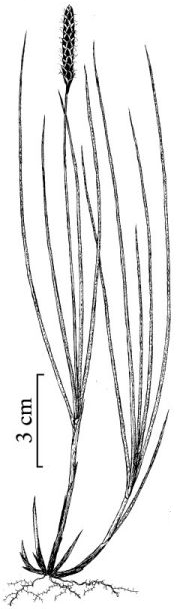
\includegraphics[scale=0.3]{images/1.png}} \\
    & \\
    \textbf{Carex scirpoidea var. convoluta} & \\
    \textbf{Carex scirpoidea convoluta Kükenth.} & \\
    \textbf{Carex scirpoidea var. convoluta Kuk.} & \\
    \textbf{Carex scirpoidea var. convoluta Kük.} & \\
    \textbf{Carex scirpoidea var. convoluta Kükenth.} & \\
    \textbf{Carex scirpoidea var. convoluta Kükenthal} & \\
    \textbf{Carex scirpoidea Michx. var. convoluta Kük.} & \\
    \textbf{Carex scirpoidea Michx. var. convoluta Kükenth.} & \\
    \textbf{Carex scirpoidea Michaux var. convoluta Kükenthal} & \\
    & \\
    \textbf{Carex scirpoidea subsp. convoluta} & \\
    \textbf{Carex scirpoidea ssp. convoluta (Kük.) Dunlop} & \\
    \textbf{Carex scirpoidea subsp. convoluta (Kük.) Dunlop} & \\
    \textbf{Carex scirpoidea ssp. convoluta (Kukenth.) Dunlop} & \\
    \textbf{Carex scirpoidea subsp. convoluta (Kük.) D.A.Dunlop} & \\
    \textbf{Carex scirpoidea subsp. convoluta (Kük.) D.A. Dunlop} & \\
    \textbf{Carex scirpoidea Michx. ssp. convoluta (Kük.) Dunlop} & \\
    \textbf{Carex scirpoidea subsp. convoluta (Kuk.) D. A. Dunlop} & \\
    \textbf{Carex scirpoidea Michx. subsp. convoluta (Kük.) Dunlop} & \\
    \textbf{Carex scirpoidea Michx. ssp. convoluta (Kükenth.) Dunlop} & \\
    \textbf{Carex scirpoidea subsp. convoluta (Kükenthal) D.A. Dunlop} & \\
    \textbf{Carex scirpoidea Michx. subsp. convoluta (Kük.) D.A.Dunlop} & \\
    \textbf{Carex scirpoidea Michx. subsp. convoluta (Kük.) D.A. Dunlop} & \\
    \textbf{Carex scirpoidea subsp. convoluta (Kükenthal 1909) D.A. Dunlop 1998} & \\
    \hline
    \end{tabular}
  \end{center}
\end{table}

Table~\ref{table:carex} illustrates that there is no single correct way to
spell scientific names. Because of such variations, less than 15\% of the names in comparisons of large biological databases could be matched based on exact spellings of name-strings \cite{Patterson:inpress-a}. In order to improve this simple metric for interoperability, we need to be able to identify such spelling variants as the same name, a process referred to as ''lexical reconciliation''.  Reconciliation involves linking alternative name-strings (whether spelling variants, nomenclatural variants, identifiers, common names, or surrogates for names) for the same taxon into
reconciliation groups. Most biologists do this intuitively - they recognize  that the name-strings in Table 1 refer to the same taxon. They do so by  ``parsing'' the name-strings into component elements (genus name, species name, authors, ranks etc.) and mentally discarding  less significant elements such as annotations and
authorship. It then becomes clear all of name-strings have a common ``canonical
form'' -- \textbf{Carex scirpoidea convoluta}. Further analysis of the
name-strings would reveal two different reconciliation groups for, probably, one concept:

\begin{itemize}

  \item \textbf{Carex scirpoidea var. convoluta} description by
    \textbf{Kükenthal}

  \item \textbf{Carex scirpoidea subsp. convoluta} rank determination by
    \textbf{Dunlop}.

\end{itemize}

The need to parse scientific names to achieve normalized names has mostly been 
addressed by manual means. A person familiar with
 rules of botanical nomenclature would be able to analyse the example of 24
name-strings with relative ease, but not thousands or millions of
name-strings to which more than one nomenclatural code may be applied. The manual splitting of names into even two parts, the latinized elements elements of taxon names that make up the canonical form and the
authorship is expensive, slow, inflexible. To scale this exercise up and to address such edge cases requires an algorithmic solution, a scientific name parser!

The strategy of the algorithmic approach is to identify which combinations of the most atomic elements of a name-string (i.e. the UTF-8 encoded characters) represent words (such as genus name, species name, authors, annotations) or dates.  An early algorithmic approach to parsing scientific names was with regular
language implemented as regular expression \cite{Leary2007}. A regular expression
is a sequence of characters that describes a search pattern
\cite{aho1992foundations}. For example, a regular expression ``[A-Z][a-z]\{2\}''
recognizes any capitalized word that starts from a capital letter proceeded by two small letters (e.g. ``Zoo''). Scientific names almost universally follow patterns such as the use of spaces to separate words, capitalization (of generic names and authors) or the inclusion of four digit dates between the middle of the 18th century and the present dates scientific names. This makes most names amenable to parsing by regular expressions.  Examples of
parsers based on regular expressions are GBIF's \textit{name-parser}
\cite{gbifNameParser}, and \textit{YASMEEN} \cite{VandenBerghe2015}.

While regular expression is a powerful approach to string parsing,  it has
limitations. It cannot elegantly deal with name-strings where an authorship element is present in the middle of the name (for example
\textbf{Carex scirpoidea Michx. subsp.  convoluta (Kük.) D.A.Dunlop}).  Indeed regular expressions are not well suited to any targets 
with recursive (nested) elements \cite{yu1997handbook}, such as hybrid formulae (e.g. \textbf{Brassica oleracea L.
subsp.  capitata (L.) DC. convar. fruticosa (Metzg.) Alef.  $\times$ B.
oleracea L. subsp. capitata (L.) var.  costata DC.}). Name parsing built on
regular expressions is impractical for complex name-strings.

Another limitation with most regular expression software tools is that they are ``black
boxes'' that allow limited interaction with the parsing process, and do not reveal much information about the parsing context. Developers cannot call a
procedure during a parsing event. As a result they are difficult to implement and maintain some functions such as error recovery, detailed warnings, and descriptions of errors.

We wanted an approach able to deal with the most complex scientific names of broader
complexity to give more flexibility than can be achieved with a regular expression approach.  We
believe that a general use parser should satisfy the following requirements.

\begin{enumerate}

  \item \textbf{High Quality.} A parser should be able to break names into
    their semantic elements to the same standards that can be achieved by a
    trained nomenclaturalist or better. This will give users confidence in the
    automated process and allow them to set aside  tedious and expensive manual parsing.

  \item \textbf{Global Scope.} A parser should be able to parse all types of
    scientific names, inclusive of the most complex name-strings such as hybrid
    formulae, multi-infraspecific names, names with multilevel authorships and so on.   No name-strings should be left unparsed, otherwise information attached to
    them may remain undiscoverable.

  \item \textbf{Parsing Completeness.} All information included in a
    name-string is important, not only the canonical form of the scientific
    name. Authorship, year, rank information allow us to distinguish homonyms,
    similar names, synonyms, spelling mistakes, or chresonyms.  Access to such information  improves the performance of subsequent reconciliation.

  \item \textbf{Speed.} Users, especially large-scale aggregators of  biodiversity data, are more satisfied with quick responses, as it allows them to move onto to more purposeful value-adding tasks.  Speed reduces the costs of building or running the hardware used for parsing. 

  \item \textbf{Accessibility.} To be available to the widest possible audience
    a parser should be released as a stand-alone program,  have a good
    documentation, be able to work as a library, to function as a command line tool, as a tool within a graphical interface, and to run as a socket or as RESTful services.

\end{enumerate}

These requirements became our design goals. Based on our experience with
prototype systems, we selected Parsing Expression Grammars and Scala language for the following reasons.

\subsection*{Adoption of Parsing Expression Grammars}

Parsing Expression Grammars (PEG) \cite{Ford2004} have been recently introduced for parsing strings. PEG allows users to define the rules (``grammar'') which describe general structure
of target strings. In our case, such rules can be used to deconstruct scientific names.
The rules are built from the ground up, staring from the simplest -- what UTF-characters refer to a ``character'' or ``space''.  That process will identify most 'words'.  Characters can be divided into digits and other characters to make dates identifiable. Further rules can be applied, such as a ``genus'' rule would be a name-string in which the first word begins with combination of a
``capital\_character'' followed by several ''lower\_case\_characters'' that fall within a relatively small spectrum of latinized letters;  
``authorship'' would be one or a combination of capitalized words and optionally a ``year'' within, in some cases, authors grouped to form author-teams. PEG rules are designed to be recursive. They can be expanded to deal with increasingly complex name-strings, or address  errors such as absent spaces, extra spaces, or OCR errors. Each rule can have programmatic logic attached, making the PEG approach very flexible. We believe that PEG suits our goals
better than regular expressions for the following reasons:

\begin{itemize}

  \item PEG is better suited to strings with recursive structure than, for example, regular expressions;

  \item the syntax of scientific names' is formal enough to be closer to an algebraic
    structure rather than to a natural language. Inconsistencies and
    ambiguities in scientific names are relatively rare due to compliance with the conventions of nomenclatural codes;

  \item scientific name-strings are short enough to avoid problems with
    computational complexity and memory consumption;

  \item programming a parser is easier than regular expressions because
    PEG allows parsing rules in domain-specific language; and

  \item domain specific language offers great flexibility for logic within
    the rules, for example reporting errors in name-strings.

\end{itemize}

In 2008, Global Names created a specialized parsing library
\textit{biodiversity} \cite{biodiversity} written in Ruby and based on PEG. We used an excellent \textit{TreeTop} Ruby library \cite{treetop} as the underlying PEG implementation.

The PEG approach allowed us to deal with complex scientific names gracefully.
It gave us flexibility to incorporate edge cases and to detect common mistakes
during the parsing process. The library \textit{biodiversity} enjoyed
considerable popularity. At the time of writing, it had been downloaded more
than 150,000 times \cite{bdiv-downloads}, it is used by many taxon name
resolution projects (e.g. Encyclopedia of Life \cite{eol}, Canadian Register of
Marine Species (CARMS) \cite{carms}, the iPlant TNRS \cite{iplant}, and World
Registry of Marine Species (WoRMS) \cite{worms}.  According to statistics compiled by BioRuby, \textit{biodiversity}, at the time of writing, has been the most
popular bio-library in the Ruby language \cite{biogems}.

We were pleased with PEG approach for scientific names parsing, but now regard
the \textit{biodiversity} parser library as a working prototype. It has  allowed us
to identify problems and implement improvements in order to build a production parser.

\subsection*{Adoption of Scala}

The \textit{biodiversity} package had performance and scalability issues because
of the choice of Ruby as its programming language. Ruby is one of the best
languages for rapid prototyping, but it is an interpreted dynamic language with,
originally, a single-threaded runtime in a virtual machine. This makes it slow
and inappropriate for rapid service or large tasks. We determined that we
needed an environment with the following properties:

\begin{itemize}

    \item a mature technology;

    \item able to be multi-threaded, with high performance and scalability;

    \item an active support community with open-source friendly culture;

    \item a wide range of libraries: utilities, web frameworks, etc.;

    \item a mature development environment with IDEs, testing frameworks, debuggers,  profilers and the like;

    \item using technologies for search and cluster computations;

    \item interoperable with languages used in scientific community (R,
      Python, Matlab); and

    \item natural support of domain specific languages embedded in the hosted
      language.

\end{itemize}

While many of the properties are true for Ruby, others, such as high
performance, scalability and interoperability are lacking. To meet all
requirements, and exploiting what we had learned from \textit{biodiversity}, we
refactored the code to fulfil all our requirements using the Java virtual machine, Scala
programming language \cite{odersky2004overview}, and the Open Source
\textit{parboiled2} library \cite{parboiled2} which implements PEG in Scala. An
alternative to \textit{parboiled2} is the Scala parser combinators library
\cite{moors2008parser} but it has known problems with speed and memory consumption
making \textit{parboiled2} our preferred choice. The functional programming features of Scala allowed us to build a custom
parsing language that describes the rules of the grammars of scientific names.
This produces a Parsing Expression Grammar with considerably more
flexibility than external Lexers such as Bison or Yacc. As this domain specific
language is within \textit{parboiled2} it can take advantage of the Macro
capacity of Scala \cite{Burmako:2013:SML:2489837.2489840} to modify the
compiler and how the program operates. The result is that the software operates
with high efficiency. With this combination, the resulting \textit{gnparser} achieved a significant
boost in speed, scalability, and portability of the library.  We limited this
version to work with scientific names that comply with the botanical,
zoological, and prokaryotic codes of nomenclature, but not with names of viruses because they are
formed in different ways \cite{ICTV, Patterson:inpress-a} and will need a different PEG.

\section*{Implementation}

The \textit{gnparser} project is entirely written in Scala. It supports two
major Scala versions: 2.10.6+ and 2.11.x. The code is organized into four
modules:

\begin{enumerate}

  \item ``\textit{parser}'' is the core module used by all other modules. It
    contains the components for parsing of scientific names from the most atomic elements to semantically-defined terms. It includes the parsing
    grammar, abstract syntax tree (AST) composed of the components of scientific names, warnings and error facilities.  When the
    parsing is complete and semantic elements of name-strings have been assigned to AST nodes, 
    then the elements can be recombined and formatted to meet further needs.  For
    example:

\begin{itemize}

  \item \textit{normalizer} can convert input name-strings into a consistent style;

  \item \textit{canonizer} creates canonical forms of the latinized elements of names; and with

  \item \textit{JSON renderer}, the parsing result is converted to JSON
    \cite{bray2014javascript} to allow developers to work with the output from other languages. The output (figure 1, also see Discussion) has the following information: \textbf{details} contains the JSON-representation of a parsed scientific name; \textbf{quality\_warnings} describes potential problems if names are not well-formed; \textbf{quality} depicts a quality level of the parsed name;  and \textbf{positions} maps the positions of every element in a parsed name to the semantic meaning of the element. Full and formal explanation of all parser fields is given as a JSON schema
can be found online \cite{gnparser-json}.

\end{itemize}

  \item ``\textit{examples}'' contains  examples to assist developers in
    building \textit{parser} into other popular programming languages such as Java,
    Scala, Jython, JRuby, and R.

  \item ``\textit{runner}'' contains the code that allows users to run
    ``\textit{parser}'' from a command line as a standalone tool or to run it
    as a TCP/IP socket server. ``\textit{runner}'' depends on the
    ``\textit{parser}''.   The core part is the launch script
    ``\textit{gnparse}'' (for Linux/Mac and Windows) that creates a JVM instance
    and runs ``\textit{parser}'' on multiple threads against the input provided
    via a socket or file.

  \item ``\textit{web}'' contains a web application and a RESTful interface as
    simpler methods to access ``\textit{parser}''. It is a Play Framework
    \cite{wampler2011scala} application. It depends on the ``\textit{parser}''
    library. ``\textit{web}'' achieves interactions with ``\textit{parser}''
    via HTTP protocols. It works both with simple HTML and REST API interfaces
    Figure~\ref{figure:webgui} illustrates a parsing example using the web-interface.

\end{enumerate}

All subprojects except ``\textit{web}'' can run in JVM 1.6. ``\textit{web}''
requires JVM 1.8. Documentation is available in a README file (see section ``Availability and Requirements).

\begin{figure}[htbp]
  \begin{center}

    \caption{Web Graphical User Interface \cite{gnparser-web}. In this example
      a user entered a name-string of a hybrid name consisted of 21 elements.
      The ``Results'' section contains detailed parsed output using compact
      JSON format.}\label{figure:webgui}

    \vspace{5mm}
    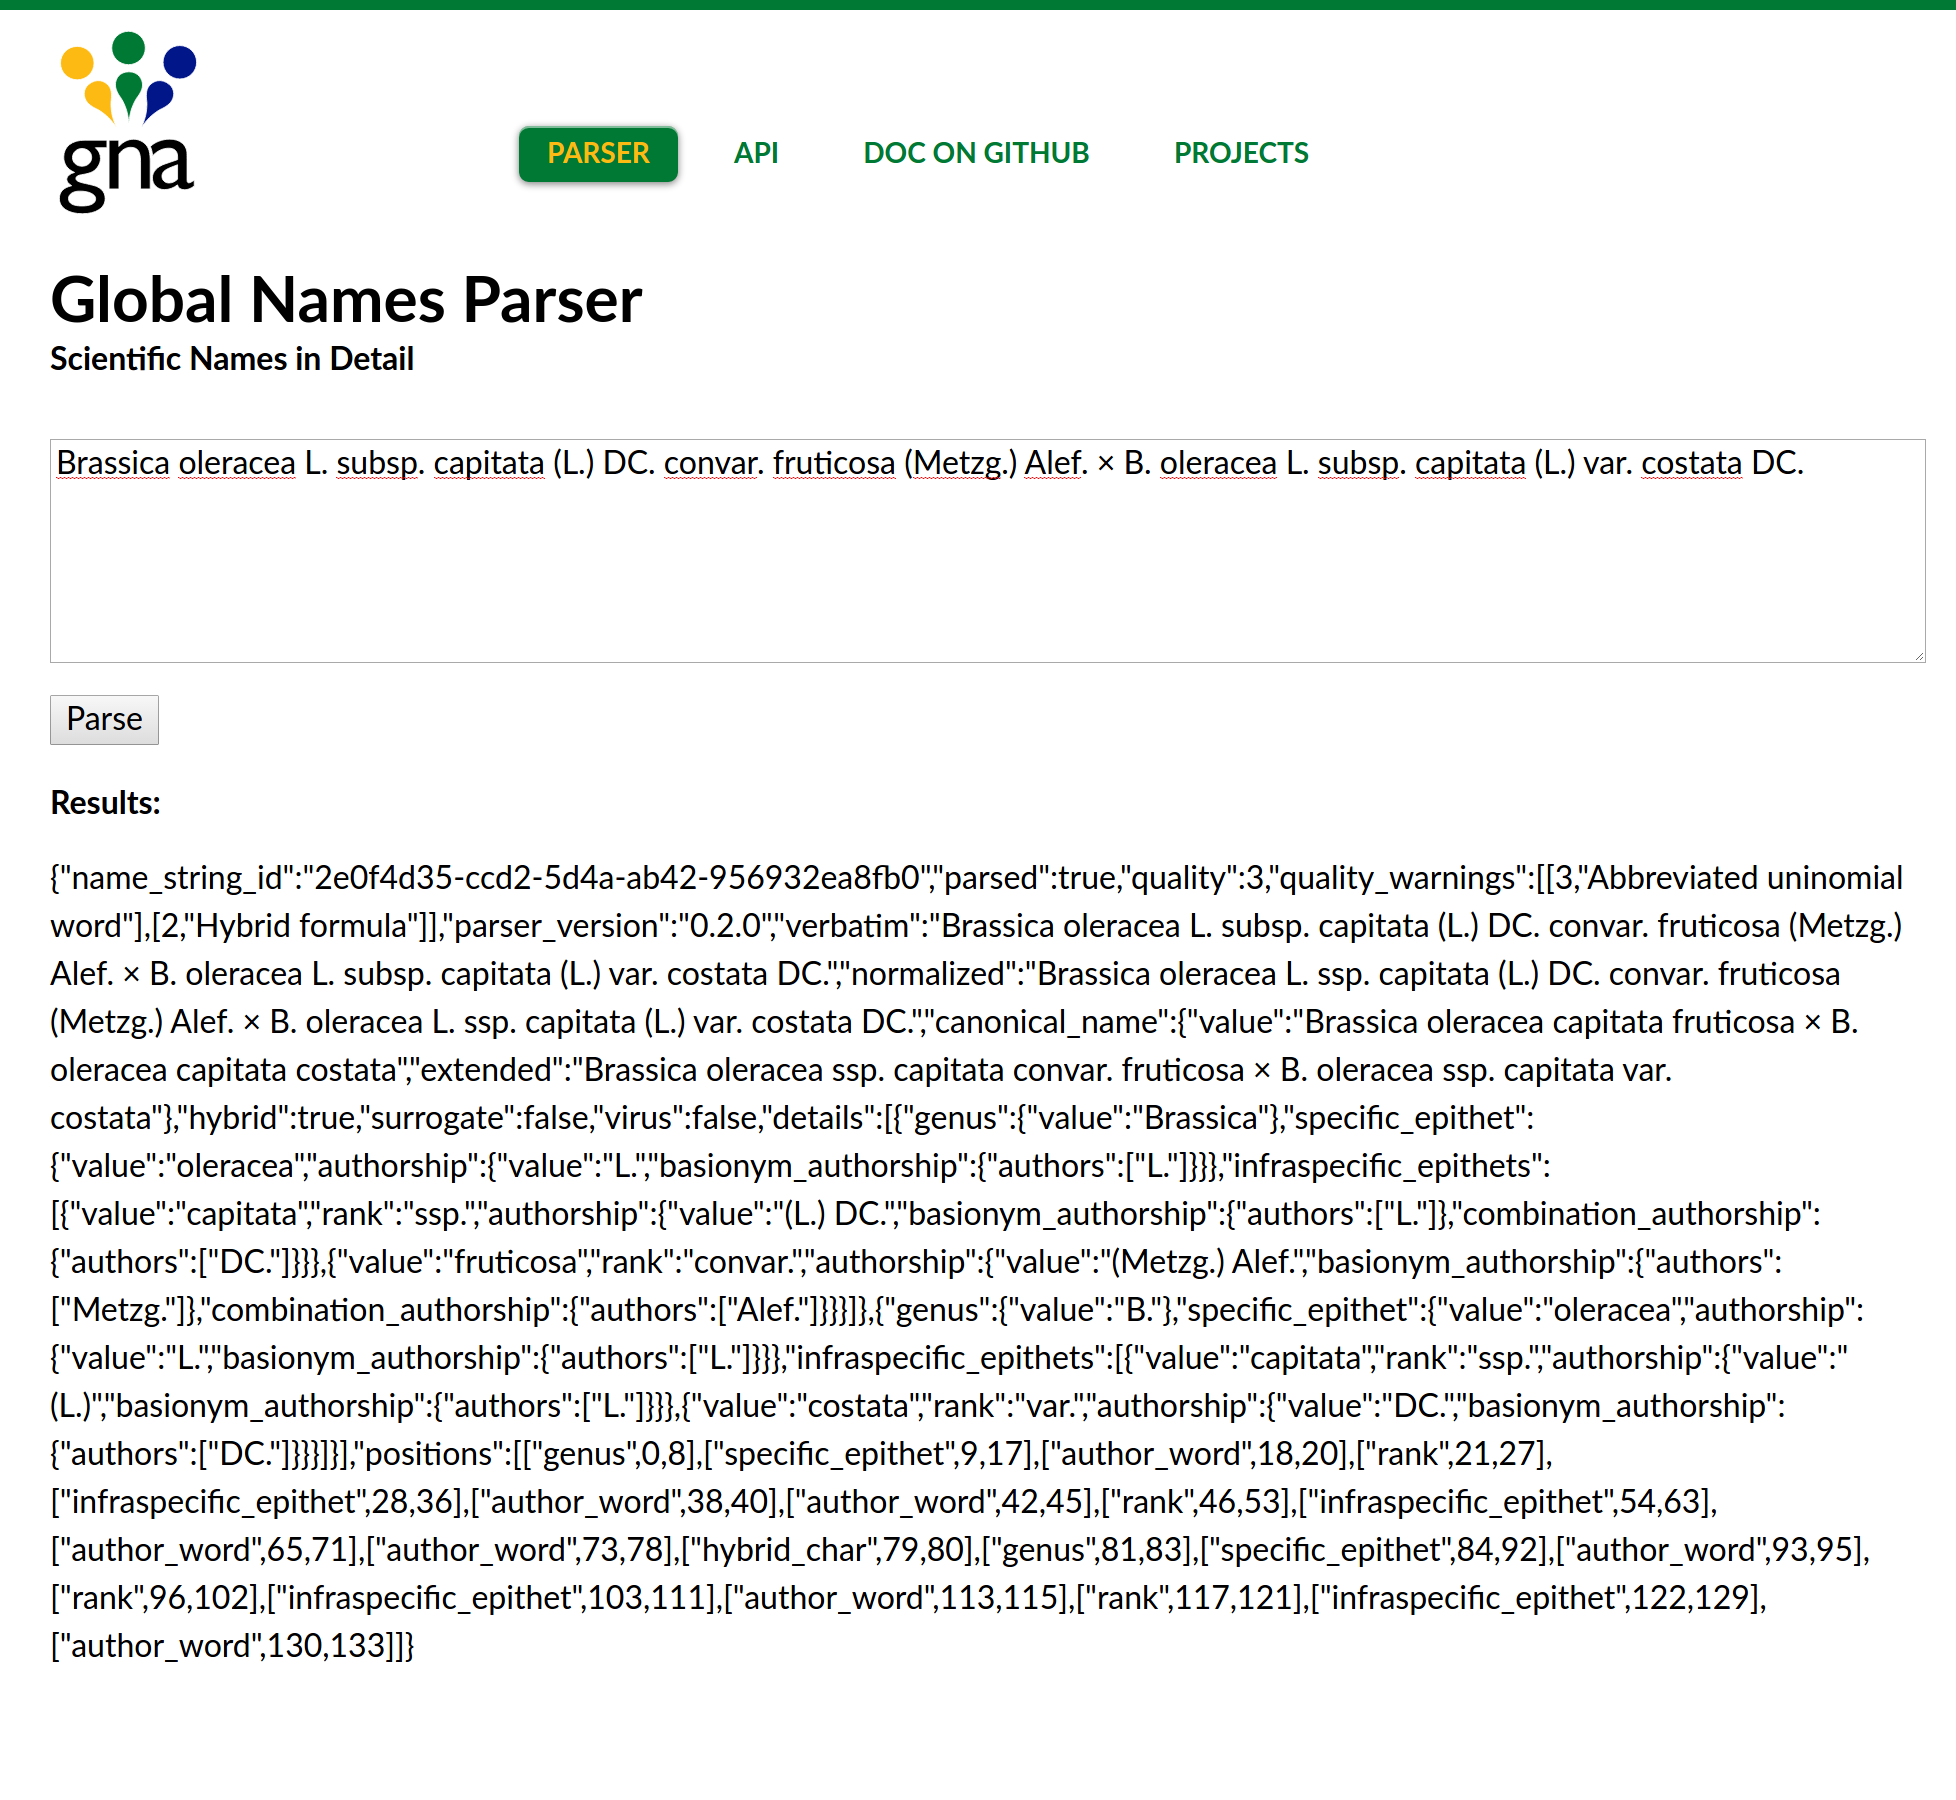
\includegraphics[scale=0.175]{images/2.png}
  \end{center}
\end{figure}

\subsection*{Installation}

``\textit{gnparser}'' is available for launch in three bundles.

\begin{itemize}
%comment paddy, two references required below
  \item A \textit{parser} artifact is provided via the Maven central repository of
    Java code \cite{maven-globalnames}. Physically it is a relatively small jar file without
    embedded external dependencies. The artifact can be accessed by a build system such
    as Maven, Gradle, or SBT in custom projects. The build system then
    identifies and provides access to all dependent jars.

  \item A Zip-archived ``fat jar'' is located at the project's GitHub
    repository. The jar contains the compiled files of \textit{gnparser} along
    with all necessary dependencies to launch it within JVM. The archive is
    also bundled with a launch script (for Windows, OS X and Linux) that can
    run a command line interface to \textit{gnparser}.

  \item The project's Docker container is located at Docker hub  (REFERENCE REQUIRED!).
    Docker provides an additional layer of abstraction and automation of
    operating-system-level virtualization on Linux. It can be thought as
    lightweight virtualization technology within same Linux OS process. When it
    is setup properly, everything -- starting from JVM and ending with Scala
    and SBT -- can be run with simple commands that will, for example,  pull
    the Docker image from the Hub, and run the socket or web server on an appropriate port.

\end{itemize}

\subsection*{Testing Methods}

Data for our tests were packages of 1,000 and 100,000 name-strings randomly chosen from
24 million name-strings of the Global Names Index \cite{gn:index}. The 
resulting datasets consisted of strings acquired from a variety of data sources
and were a mixture of well-formed names, names with formatting and spelling
mistakes, and name-strings that were misrepresented as names.

We compared performance of \textit{gnparser} with 2 other projects:
\textit{biodiversity} parser \cite{Boyle2013, biodiversity} (also developed by
Global Names), and GBIF \textit{name-parser} \cite{gbifNameParser}. For
comparison, we calculated $Precision$, $Recall$ and $Accuracy$ (as described
below) using a dataset consisted of 1000 name-strings. Another project we
considered was the YASMEEN parser from iMarine  \cite{VandenBerghe2015}. We found that with our dataset it generated dramatically more mistakes
than other parsers ($Precision$ 0.534, $Recall$ 1.0, $F1$ 0.6962), and was
unable to finish a full dataset without crashing. We excluded it from further tests.

To estimate the quality of the parsers being compared, we used a
combination of canonical form and terminal authorship as this is a feature that  common to all three parsers.  A canonical form
represents the essential scientific elements of a name, while the terminal authorship
refers to the author of the lowest subtaxon referred to in the name. For
example, with \textbf{Oriastrum lycopodioides Wedd.  var.  glabriusculum Reiche}, the
canonical form is \textbf{Oriastrum lycopodioides glabriusculum} and the terminal
authorship is \textbf{Reiche}, not \textbf{Wedd.}.

 When both the canonical form and the terminal authorship were determined
correctly we marked the result as true positive ($N_{tp}$).  If one or both
of them were determined incorrectly, the result was marked a false positive
($N_{fp}$). Name-strings correctly discarded from parsing were marked as
true negatives ($N_{tn}$). False negatives ($N_{fn}$) were ``suitable''
name-strings which should be parsed, but were not The
following parameters where used for analysis:

$Accuracy$ -- the proportion of correct results to all results.  It is calculated
as:

\[Accuracy = \dfrac{N_{tp} + N_{tn}}{N_{tp} + N_{tn} + N_{fp} + N_{fn}}\]

$Precision$ -- the proportion of name-strings parsed correctly compared to all detected
name-strings. It is is calculated as:

\[Precision = \dfrac{N_{tp}}{N_{tp} + N_{fp}}\]

$Recall$ -- the proportion of correctly detected name-strings relative to all parseable
name-strings and calculated as:

\[Recall = \dfrac{N_{tp}}{N_{tp} + N_{fn}}\]

$F1-measure$ is a balanced harmonic mean (where $Precision$ and $Recall$ have
the same weight). When $Precision$ and $Recall$ differ, $F1-measure$ allows
results to be compared. It is calculated as

\[F1 = \dfrac{2 \times Precision \times Recall}{Precision + Recall}\]


Some names in the dataset were not well-formed. If a human could extract the
canonical form and the terminal authorship from them, we included them.
Examples of such name-strings are \textbf{"Bumetopia (bumetopia) quadripunctata
Breuning"} (the issue here is the lower case initial letter of the subgenus), \textbf{"Campylium
gollanii C. M?ller ex Vohra 1970 [1972]"} (with a miscoded UTF-8 symbol and an
additional year in square brackets), \textbf{"Myosorex muricauda (Miller,
1900)."} (with a period after the authorship).

Parsers analyze the structure of name-strings, but they cannot determine if
a string is a ``real'' name. For example, in the case of a name-string that has
the same form as a subspecies such as \textbf{"Example name Word var. something
Capitalized Words, 1900"}. In such a case, the identification of a canonical
form as \textbf{"Example name something"} and terminal authorship as
\textbf{"Capitalized Words, 1900"} would be considered a true positive. Clearly, it will be important for name-management services to  distinguish between name-strings of
scientific names, names of viruses, surrogate names, and non-names. To find out
how well parsers distinguished strings which are not scientific names, we
calculated $Precision$ for discarded/non-parsed strings. If done correctly,
not-parsed strings would include only names of viruses and terms that do not
comply with the Codes of zoological, prokaryotic, and botanical nomenclature.

We processed 100,000 name-strings with each parser.  Each parser discarded
close to 1000 name-strings as not-parseable.  $Precision$ in this case showed
percentage of correctly discarded names.  We do not know $Recall$, as it was
not reasonable to manually determine this for 100,000 names. To get a sense of
names which should be discarded but were parsed instead, we analysed
intersections and differences of the results between the three parsers.

To establish the throughput of parsing we used a computer with an Intel
i7-4930K CPU (6 cores, 12 threads, at 3.4 GHz), 64GB of memory, and 250GB
Samsung 840 EVO SSD, running Ubuntu version 14.04. Throughput was determined by
processing of 1,000,000 random name-strings from GNI.

To study the effects of parallel execution on throughput we used the
\textit{ParallelParser} class from \textit{biodiversity} parser and
\textit{gnparse} a command line interface for \textit{gnparser}. For GBIF
\textit{name-parser}, we created a thin wrapper with multi-threaded
capabilities \cite{gbifparser}.

\section*{Results and Discussion}

We discuss and compare \textit{gnparser}, GBIF \textit{name-parser} and
\textit{biodiversity} parser in terms of our requirements of
quality, global scope, parsing completeness, speed, and accessibility. 


\subsection*{High Quality Parsing}

Quality is the most important  of the 5 requirements.  We
compared \textit{gnparser} together with 2 other approaches  that
represent state of the art for parsing biological scientific names. GBIF
\textit{name-parser} uses regular expressions approach, while \textit{gnparser}
and \textit{biodiversity} parsers use PEG approach.  Results for quality
measurements are shown in Table~\ref{table:precision}.

If test data contain a large proportion of true negatives ($N_{tn}$)
$Accuracy$ will not be a good measure as it favors algorithms which distinguish
negative results, rather than finding positive ones. We manually checked our test datasets and established that  $\approx1\%$ were not scientific names. Given that true negatives are rare, they will have very limited influence on $Accuracy$. $Recall$ for all parsers was high, which means that false negatives are not important. 

We hold that $Accuracy$ is probably the best measure
for our tests. All 3 parsers performed very well, with $Accuracy$
values higher than $95\%$. Both \textit{gnparser} and \textit{biodiversity}
parser approached 99\% mark which we regard as production quality. Moreover,
most of the false positives came from name-strings with mistakes. For example, out of 11 false positives (below) that \textit{gnparser} found in the 1000
name-string test data set, only 2 (the first 2) were well-formed names. 

\vspace{0.5cm}
%comment Paddy: Dma, can you boldface these examples (and any other lists of examples)
\begin{verbatim} 
    Eucalyptus subser. Regulares Brooker}
    Jacquemontia spiciflora (Choisy) Hall. fil.

    Acanthocephala declivis variety guianensis Osborn, 1904
    Atysa (?) frontalis
    Bumetopia (bumetopia) quadripunctata Breuning, 1950
    Cyclotella kã¼tzingiana Thwaites
    Elaphidion (romaleum) tæniatum Leconte, 1873
    Hieracium nobile subsp. perclusum (Arv. -Touv. ) O. Bolòs & Vigo
    Leptomitus vitreus (Roth) Agardh{?}
    Myosorex muricauda (Miller, 1900).
    Papillaria amblyacis (M<81>ll.Hal.) A.Jaeger}
\end{verbatim}

\vspace{0.5cm}

We do expect a parser to deal with names that are not well-formed. That means overcoming problems such as aberrant characters which might arise from Unicode character miscodings, inappropriate annotations, or other mistakes. To alert users,
\textit{gnparser} generates a warning when it identifies a problem in a name-string. The other parsers do not have this feature.

When parsers reach $\approx80\%$ $Accuracy$, they hit a ``long tail'' of
problems where each particular type of a problem is rare, yet every new manual
test against a new test set of 1,000-10,000 name-strings reveals new issues.  Examples of these
challenges are given elsewhere \cite{Patterson:inpress-a}. For all three
parsers, developers had to perform the meticulous task of adding rules to address one rare case after
another. That is, parsers need to be subject to continuous improvement. The problems found
during preparation of this paper are being addressed in the next version of
\textit{gnparser}. As the parsing rules improve, we believe that
\textit{gnparser} can reach $>99.5\%$ $Accuracy$ without diminishing $Recall$.

As we incorporate new rules to increase $Recall$, we have to consider the risks
of reducing $Precision$ by introducing new false positives. For example, the GBIF
\textit{name-parser} allows the genus element of a name-string to start with a
lowercase character. As a result the name-strings below were parsed as if they
were scientific names, while other parsers ignored them:

\vspace{0.5cm}

\begin{verbatim}
    acid mine drainage metagenome
    agricultural soil bacterium CRS5639T18-1
    agricultural soil bacterium SC-I-8
    algal symbiont of Cladonia variegata MN075
    alpha proteobacterium AP-24
    anaerobic bacterium ANA No.5
    anoxygenic photosynthetic bacterium G16
    archaeon enrichment culture clone AOM-SR-A23
    bacterium endosymbiont of Plateumaris fulvipes
    bacterium enrichment culture DGGE band 61_3_FG_L
    barley rhizosphere bacterium JJ-220
    bovine rumen bacterium niuO17
\end{verbatim}

\vspace{0.5cm}

Strategies like these might increase $Recall$ with certain low-quality datasets,
but they decrease $Precision$. Many
``dirty'' datasets contain recurring problems. As an example, DRYAD contains many name-strings in which elements of scientific names are concatenated with an interpolated character such as `\_’ (e.g. ``Homo\_sapiens'' and ``Pinoyscincus\_jagori\_grandis'') \cite{Patterson:inpress-a}. For them, our solution
was to include a ``preparser'' script which ``normalizes'' known problems that are inherent within that dataset and
then apply a high quality parser to the result.  

Our testing also revealed differences between regular expressions and PEG
approaches. Both can achieve high quality results with canonical forms of scientific names, but the
regular expressions are less suitable for more complex name-strings. The reason for this is the recursive or nested nature of some scientific names that lead to greater
problems that at some point become unsurmountable for regular expressions.

\subsection*{Global Scope}

If we want to connect biological data using scientific names, no name-strings
should be missed or rejected, no matter how complex they are. During our
testing we found that $Accuracy$ of GBIF's \textit{name-parser} was negatively
affected because of how it managed (or did not manage) hybrid formulae and infrasubspecific names (names
with more then one infraspecific epithet). This is where the regular expression approach reveals its limitations.  For example the following names were not parsed by the GBIF \textit{name-parser}:

\vspace{0.5cm}

\begin{verbatim}
    Crataegus chlorosarca subtaxon pubescens E.L.Wolf
    Erigeron peregrinus ssp.callianthemus var. eucallianthemus
    Salvelinus fontinalis x Salmo gairdneri
    Echinocereus fasciculatus var. bonkerae × E. fasciculatus
      var. fasciculatus
\end{verbatim}

\vspace{0.5cm}

The PEG approach supports nested parsing rules to create progressively more complex rules that do manage such examples. Its capacity to address
recursion allows \textit{gnparser} to handle the full spectrum of scientific names that we have presented to it.

\begin{table}[htb]
  \begin{center}
    \caption{Precision/Recall for parsers applied to 1000
    name-strings}\label{table:precision}
    \resizebox{10cm}{!} {
    \begin{tabular}{|l|*{3}{l}|}
      \hline
                             & gnparser & gbif-parser & biodiversity \\
      \hline
      \textit{True Positive} & 976      & 955         & 971          \\
      \textit{True Negative} & 13       & 12          & 13           \\
      \textit{False Positive}& 11       & 32          & 16           \\
      \textit{False Negative}& 0        & 1           & 0            \\
      \textit{Precision}     & 0.9888551& 0.967578    & 0.9837893    \\
      \textit{Recall}        & 1.0      & 0.998954    & 1.0          \\
      \textit{F1}            & 0.9943963& 0.983016    & 0.9918284    \\
      \textit{Accuracy}      & 0.989    & 0.967       & 0.984        \\
      \hline
    \end{tabular}
    }
  \end{center}
\end{table}

\begin{table}[htb]
  \begin{center}
    \caption{Precision for discarded by parsers names, out of 100 000
    name-strings}\label{table:unparsed}
    \resizebox{10cm}{!} {
    \begin{tabular}{| l | *{3}{l} |}
      \hline
                              & gnparser & gbif-parser & biodiversity \\
      \hline
      \textit{Total discarded}& 1131     & 1082        & 1161         \\
      \textit{True Positive}  & 1129     & 940         & 1152         \\
      \textit{False Positive} & 2        & 142         & 9            \\
      \textit{Precision}      & 0.998231 & 0.868761    & 0.9922481    \\
      \hline
    \end{tabular}
  }
  \end{center}
\end{table}

\begin{figure}[htbp]
  \begin{center}
    \caption{
      Names parsed per second by GN, GBIF and Biodiversity parsers
      (running on 1-12 parallel threads).
    }\label{figure:throughput}
    \vspace{0.5cm}
    \begin{tabular}{| l | *{3}{r} | c c c |}
      \hline
      \multirow{1}{*}Threads & gnparser & gbif-paser & biodiversity
      & \multicolumn{3}{c |}{Ratio} \\
      \cline{5-7}
      & & & & gn & gbif & bio \\
      \hline
      1  & 5944  & 6389  & 1111 & 1 & 1.07 & 0.19 \\
      2  & 11416 & 12638 & 1722 & 1 & 1.11 & 0.14 \\
      4  & 20500 & 21994 & 2556 & 1 & 1.07 & 0.12 \\
      8  & 24805 & 30972 & 2777 & 1 & 1.25 & 0.11 \\
      12 & 26055 & 31833 & 2527 & 1 & 1.22 & 0.10 \\
      \hline
    \end{tabular}
    % Created by tikzDevice version 0.9 on 2015-12-21 16:35:00
% !TEX encoding = UTF-8 Unicode
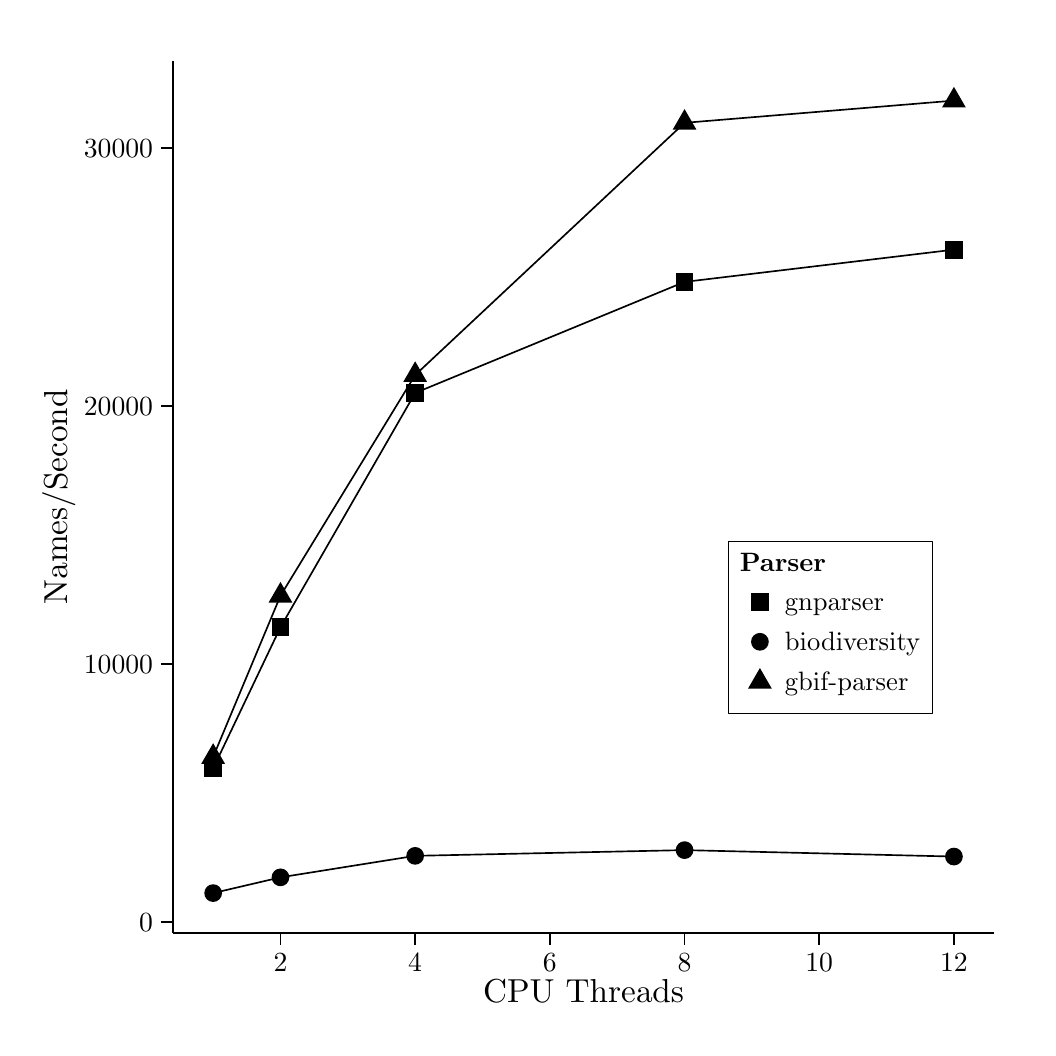
\begin{tikzpicture}[x=1pt,y=1pt]
\definecolor{fillColor}{RGB}{255,255,255}
\path[use as bounding box,fill=fillColor,fill opacity=0.00] (0,0) rectangle (361.35,361.35);
\begin{scope}
\path[clip] (  0.00,  0.00) rectangle (361.35,361.35);
\definecolor{drawColor}{RGB}{255,255,255}
\definecolor{fillColor}{RGB}{255,255,255}

\path[draw=drawColor,line width= 0.6pt,line join=round,line cap=round,fill=fillColor] (  0.00,  0.00) rectangle (361.35,361.35);
\end{scope}
\begin{scope}
\path[clip] ( 52.42, 34.31) rectangle (349.30,349.30);
\definecolor{fillColor}{RGB}{255,255,255}

\path[fill=fillColor] ( 52.42, 34.31) rectangle (349.30,349.30);
\definecolor{drawColor}{RGB}{255,255,255}

\path[draw=drawColor,line width= 0.6pt,line join=round] ( 52.42, 38.27) --
	(349.30, 38.27);

\path[draw=drawColor,line width= 0.6pt,line join=round] ( 52.42,131.48) --
	(349.30,131.48);

\path[draw=drawColor,line width= 0.6pt,line join=round] ( 52.42,224.69) --
	(349.30,224.69);

\path[draw=drawColor,line width= 0.6pt,line join=round] ( 52.42,317.90) --
	(349.30,317.90);

\path[draw=drawColor,line width= 0.6pt,line join=round] ( 91.35, 34.31) --
	( 91.35,349.30);

\path[draw=drawColor,line width= 0.6pt,line join=round] (140.02, 34.31) --
	(140.02,349.30);

\path[draw=drawColor,line width= 0.6pt,line join=round] (188.69, 34.31) --
	(188.69,349.30);

\path[draw=drawColor,line width= 0.6pt,line join=round] (237.36, 34.31) --
	(237.36,349.30);

\path[draw=drawColor,line width= 0.6pt,line join=round] (286.03, 34.31) --
	(286.03,349.30);

\path[draw=drawColor,line width= 0.6pt,line join=round] (334.70, 34.31) --
	(334.70,349.30);
\definecolor{drawColor}{RGB}{0,0,0}

\path[draw=drawColor,line width= 0.6pt,line join=round] ( 67.02, 48.63) --
	( 91.35, 54.32) --
	(140.02, 62.09) --
	(237.36, 64.16) --
	(334.70, 61.83);

\path[draw=drawColor,line width= 0.6pt,line join=round] ( 67.02, 97.82) --
	( 91.35,156.08) --
	(140.02,235.82) --
	(237.36,326.96) --
	(334.70,334.99);

\path[draw=drawColor,line width= 0.6pt,line join=round] ( 67.02, 93.68) --
	( 91.35,144.69) --
	(140.02,229.35) --
	(237.36,269.48) --
	(334.70,281.13);
\definecolor{fillColor}{RGB}{0,0,0}

\path[fill=fillColor] ( 63.82, 90.48) --
	( 70.22, 90.48) --
	( 70.22, 96.88) --
	( 63.82, 96.88) --
	cycle;

\path[fill=fillColor] ( 88.15,141.48) --
	( 94.55,141.48) --
	( 94.55,147.89) --
	( 88.15,147.89) --
	cycle;

\path[fill=fillColor] (136.82,226.15) --
	(143.22,226.15) --
	(143.22,232.55) --
	(136.82,232.55) --
	cycle;

\path[fill=fillColor] (234.16,266.28) --
	(240.56,266.28) --
	(240.56,272.68) --
	(234.16,272.68) --
	cycle;

\path[fill=fillColor] (331.50,277.93) --
	(337.90,277.93) --
	(337.90,284.33) --
	(331.50,284.33) --
	cycle;

\path[fill=fillColor] ( 67.02,102.80) --
	( 71.33, 95.33) --
	( 62.71, 95.33) --
	cycle;

\path[fill=fillColor] ( 91.35,161.06) --
	( 95.66,153.59) --
	( 87.04,153.59) --
	cycle;

\path[fill=fillColor] (140.02,240.80) --
	(144.33,233.33) --
	(135.71,233.33) --
	cycle;

\path[fill=fillColor] (237.36,331.94) --
	(241.67,324.47) --
	(233.05,324.47) --
	cycle;

\path[fill=fillColor] (334.70,339.96) --
	(339.01,332.50) --
	(330.39,332.50) --
	cycle;

\path[fill=fillColor] ( 67.02, 48.63) circle (  3.20);

\path[fill=fillColor] ( 91.35, 54.32) circle (  3.20);

\path[fill=fillColor] (140.02, 62.09) circle (  3.20);

\path[fill=fillColor] (237.36, 64.16) circle (  3.20);

\path[fill=fillColor] (334.70, 61.83) circle (  3.20);
\end{scope}
\begin{scope}
\path[clip] (  0.00,  0.00) rectangle (361.35,361.35);
\definecolor{drawColor}{RGB}{0,0,0}

\path[draw=drawColor,line width= 0.6pt,line join=round] ( 52.42, 34.31) --
	( 52.42,349.30);
\end{scope}
\begin{scope}
\path[clip] (  0.00,  0.00) rectangle (361.35,361.35);
\definecolor{drawColor}{RGB}{0,0,0}

\node[text=drawColor,anchor=base east,inner sep=0pt, outer sep=0pt, scale=  1.00] at ( 45.30, 34.83) {0};

\node[text=drawColor,anchor=base east,inner sep=0pt, outer sep=0pt, scale=  1.00] at ( 45.30,128.04) {10000};

\node[text=drawColor,anchor=base east,inner sep=0pt, outer sep=0pt, scale=  1.00] at ( 45.30,221.25) {20000};

\node[text=drawColor,anchor=base east,inner sep=0pt, outer sep=0pt, scale=  1.00] at ( 45.30,314.46) {30000};
\end{scope}
\begin{scope}
\path[clip] (  0.00,  0.00) rectangle (361.35,361.35);
\definecolor{drawColor}{RGB}{0,0,0}

\path[draw=drawColor,line width= 0.6pt,line join=round] ( 48.15, 38.27) --
	( 52.42, 38.27);

\path[draw=drawColor,line width= 0.6pt,line join=round] ( 48.15,131.48) --
	( 52.42,131.48);

\path[draw=drawColor,line width= 0.6pt,line join=round] ( 48.15,224.69) --
	( 52.42,224.69);

\path[draw=drawColor,line width= 0.6pt,line join=round] ( 48.15,317.90) --
	( 52.42,317.90);
\end{scope}
\begin{scope}
\path[clip] (  0.00,  0.00) rectangle (361.35,361.35);
\definecolor{drawColor}{RGB}{0,0,0}

\path[draw=drawColor,line width= 0.6pt,line join=round] ( 52.42, 34.31) --
	(349.30, 34.31);
\end{scope}
\begin{scope}
\path[clip] (  0.00,  0.00) rectangle (361.35,361.35);
\definecolor{drawColor}{RGB}{0,0,0}

\path[draw=drawColor,line width= 0.6pt,line join=round] ( 91.35, 30.04) --
	( 91.35, 34.31);

\path[draw=drawColor,line width= 0.6pt,line join=round] (140.02, 30.04) --
	(140.02, 34.31);

\path[draw=drawColor,line width= 0.6pt,line join=round] (188.69, 30.04) --
	(188.69, 34.31);

\path[draw=drawColor,line width= 0.6pt,line join=round] (237.36, 30.04) --
	(237.36, 34.31);

\path[draw=drawColor,line width= 0.6pt,line join=round] (286.03, 30.04) --
	(286.03, 34.31);

\path[draw=drawColor,line width= 0.6pt,line join=round] (334.70, 30.04) --
	(334.70, 34.31);
\end{scope}
\begin{scope}
\path[clip] (  0.00,  0.00) rectangle (361.35,361.35);
\definecolor{drawColor}{RGB}{0,0,0}

\node[text=drawColor,anchor=base,inner sep=0pt, outer sep=0pt, scale=  1.00] at ( 91.35, 20.31) {2};

\node[text=drawColor,anchor=base,inner sep=0pt, outer sep=0pt, scale=  1.00] at (140.02, 20.31) {4};

\node[text=drawColor,anchor=base,inner sep=0pt, outer sep=0pt, scale=  1.00] at (188.69, 20.31) {6};

\node[text=drawColor,anchor=base,inner sep=0pt, outer sep=0pt, scale=  1.00] at (237.36, 20.31) {8};

\node[text=drawColor,anchor=base,inner sep=0pt, outer sep=0pt, scale=  1.00] at (286.03, 20.31) {10};

\node[text=drawColor,anchor=base,inner sep=0pt, outer sep=0pt, scale=  1.00] at (334.70, 20.31) {12};
\end{scope}
\begin{scope}
\path[clip] (  0.00,  0.00) rectangle (361.35,361.35);
\definecolor{drawColor}{RGB}{0,0,0}

\node[text=drawColor,anchor=base,inner sep=0pt, outer sep=0pt, scale=  1.20] at (200.86,  9.03) {CPU Threads};
\end{scope}
\begin{scope}
\path[clip] (  0.00,  0.00) rectangle (361.35,361.35);
\definecolor{drawColor}{RGB}{0,0,0}

\node[text=drawColor,rotate= 90.00,anchor=base,inner sep=0pt, outer sep=0pt, scale=  1.20] at ( 14.29,191.81) {Names/Second};
\end{scope}
\begin{scope}
\path[clip] (  0.00,  0.00) rectangle (361.35,361.35);
\definecolor{drawColor}{RGB}{0,0,0}
\definecolor{fillColor}{RGB}{255,255,255}

\path[draw=drawColor,line width= 0.3pt,line join=round,line cap=round,fill=fillColor] (253.09,113.49) rectangle (326.76,175.63);
\end{scope}
\begin{scope}
\path[clip] (  0.00,  0.00) rectangle (361.35,361.35);
\definecolor{drawColor}{RGB}{0,0,0}

\node[text=drawColor,anchor=base west,inner sep=0pt, outer sep=0pt, scale=  0.96] at (257.36,164.73) {\bfseries Parser};
\end{scope}
\begin{scope}
\path[clip] (  0.00,  0.00) rectangle (361.35,361.35);
\definecolor{drawColor}{RGB}{255,255,255}
\definecolor{fillColor}{RGB}{255,255,255}

\path[draw=drawColor,line width= 0.6pt,line join=round,line cap=round,fill=fillColor] (257.36,146.67) rectangle (271.82,161.12);
\end{scope}
\begin{scope}
\path[clip] (  0.00,  0.00) rectangle (361.35,361.35);
\definecolor{fillColor}{RGB}{0,0,0}

\path[fill=fillColor] (261.39,150.69) --
	(267.79,150.69) --
	(267.79,157.09) --
	(261.39,157.09) --
	cycle;
\end{scope}
\begin{scope}
\path[clip] (  0.00,  0.00) rectangle (361.35,361.35);
\definecolor{drawColor}{RGB}{255,255,255}
\definecolor{fillColor}{RGB}{255,255,255}

\path[draw=drawColor,line width= 0.6pt,line join=round,line cap=round,fill=fillColor] (257.36,132.21) rectangle (271.82,146.67);
\end{scope}
\begin{scope}
\path[clip] (  0.00,  0.00) rectangle (361.35,361.35);
\definecolor{fillColor}{RGB}{0,0,0}

\path[fill=fillColor] (264.59,139.44) circle (  3.20);
\end{scope}
\begin{scope}
\path[clip] (  0.00,  0.00) rectangle (361.35,361.35);
\definecolor{drawColor}{RGB}{255,255,255}
\definecolor{fillColor}{RGB}{255,255,255}

\path[draw=drawColor,line width= 0.6pt,line join=round,line cap=round,fill=fillColor] (257.36,117.76) rectangle (271.82,132.21);
\end{scope}
\begin{scope}
\path[clip] (  0.00,  0.00) rectangle (361.35,361.35);
\definecolor{fillColor}{RGB}{0,0,0}

\path[fill=fillColor] (264.59,129.96) --
	(268.90,122.50) --
	(260.28,122.50) --
	cycle;
\end{scope}
\begin{scope}
\path[clip] (  0.00,  0.00) rectangle (361.35,361.35);
\definecolor{drawColor}{RGB}{0,0,0}

\node[text=drawColor,anchor=base west,inner sep=0pt, outer sep=0pt, scale=  0.96] at (273.62,150.59) {gnparser};
\end{scope}
\begin{scope}
\path[clip] (  0.00,  0.00) rectangle (361.35,361.35);
\definecolor{drawColor}{RGB}{0,0,0}

\node[text=drawColor,anchor=base west,inner sep=0pt, outer sep=0pt, scale=  0.96] at (273.62,136.13) {biodiversity};
\end{scope}
\begin{scope}
\path[clip] (  0.00,  0.00) rectangle (361.35,361.35);
\definecolor{drawColor}{RGB}{0,0,0}

\node[text=drawColor,anchor=base west,inner sep=0pt, outer sep=0pt, scale=  0.96] at (273.62,121.68) {gbif-parser};
\end{scope}
\end{tikzpicture}

  \end{center}
\end{figure}

\subsection*{Parsing Completness}

The extraction of canonical forms from name-strings representing scientific
names is the most useful and widely used parsing goal. Sometimes, however, this may not be sufficient because the canonical form does not
determine a name completely.

In the example in Table~\ref{table:carex} \textbf{Carex scirpoidea convoluta}
is a canonical form for \textbf{Carex scirpoidea var. convoluta Kükenthal} and
\textbf{Carex scirpoidea ssp. convoluta (Kük.) Dunlop.} The first unparsed name-string refers to the variety \textbf{convoluta} of \textbf{Carex
scirpoidea} that had been described by \textbf{Kükenthal}. The second captures
Dunlop's reclassification of \textbf{convoluta} as a subspecies. We are not be able to distinguish between these
two different names without knowing the rank and/or the corresponding authorship.
Furthermore, it is useful to see in the second example that \textbf{(Kük.)} was the
original author and \textbf{Dunlop} was the author of the new combination.

After matching by canonical form, the ranks, authors, and "types" of authorship
help users to distinguish name-strings with similar or identical canonical names from each other.
The name-string \textbf{Carex scirpoidea Michx. var. convoluta Kükenth.} adds
new information not evident in the examples in the paragraph above, that the
species \textbf{Carex scirpoidea} was described by \textbf{Michx}.

Another area in which parsers with limited abilities can give misleading results is with
negated names \cite{Patterson:inpress-a}. In these cases, the name-string
includes some annotation or marks to indicate that the information associated with the name does NOT refer to the taxon with the scientific name that is included . Examples include \textbf{Gambierodiscus aff
toxicus} or \textbf{Russula xerampelina-like sp}.

All components of a name may be important and need to be parsed and
categorized. With \textit{gnparser}, we describe the meaning of every word in
the parsed name-string and present the results in JSON format. Parsing of \textbf{Carex
scirpoidea Michx.  subsp. convoluta (Kük.) D.A. Dunlop} gives the following
JSON output
\vspace{0.5cm}

\begin{Verbatim}[fontsize=\small]
{
  "name_string_id": "203213f3-99d1-5f5e-810a-4453c4d220cb",
  "parsed": true, "quality": 1, "parser_version": "0.2.0",
  "verbatim": "Carex scirpoidea Michx.subsp. convoluta (Kük.) D.A. Dunlop",
  "normalized": "Carex scirpoidea Michx.ssp. convoluta (Kük.) D. A. Dunlop",
  "canonical_name": {
    "value": "Carexscirpoidea convoluta",
    "extended": "Carex scirpoidea ssp. convoluta"
  },
  "hybrid": false, "surrogate": false, "virus": false,
  "details": [ {
    "genus": { "value": "Carex" },
    "specific_epithet": {
      "value": "scirpoidea",
      "authorship": { 
        "value": "Michx.", 
        "basionym_authorship": { "authors": [ "Michx." ] }
      }
    },
    "infraspecific_epithets": [ {
      "value": "convoluta", "rank": "ssp.",
      "authorship": {
        "value": "(Kük.) D. A. Dunlop",
        "basionym_authorship": { "authors": [ "Kük." ] },
        "combination_authorship": { "authors": [ "D. A. Dunlop" ] }
      }
    } ]
  } ],
  "positions": [["genus", 0, 5], ["specific_epithet", 6, 16], ["author_word", 17, 23], 
    ["rank", 24, 30 ], ["infraspecific_epithet", 31, 40], ["author_word", 42, 46],
    ["author_word", 48, 50], ["author_word", 50, 52], ["author_word", 53, 59]
  ]
}
\end{Verbatim}

\vspace{0.5cm}

The output includes the semantic meaning of all parsed elements in a name-string,
indicates if the name-string was parsed successfully, if it is a virus name, a
hybrid, or a surrogate. Surrogates are name-strings that are alternatives to
names (such as acronyms) and they may or may not include part of a scientific or
colloquial name (e.g. \textbf{Coleoptera sp. BOLD:AAV0432}). The output also
includes a statement of the position of each element in the name-string.  Last, but not least, the JSON output
contains UUID version 5 calculated from the verbatim name-string. This UUID is
guaranteed to be the same for the same name-string, promoting its use to
globally connect information and annotations.

The output usually covers every semantic element in the name-string.  The fields in the  output illustrated above have the following meanings. 

%comment Paddy.  We use both bold and italics to convey special information, and it may or may not be better for this list to NOT have bold terms (Dma - your call).  I  also recommend that the list be indented one step to the right.
\begin{description}

  \item[name\_string\_id:] UUID v5 identifier;
  \item[parsed:] whether a name-string was successfully parsed (true/false);
  \item[quality:] how well-formed a name-string is (range from 1 to 3, 1 is the best);
  \item[parser\_version:] version of a parser used;
  \item[verbatim:] name-string as was submitted to \textit{gnparser};
  \item[normalized:] name-string modified by the parser to give a normalized style;
  \item[canonical\_name:] a special form of normalization that includes only the scientific elements of the name, this form is contained within most name-strings;
  \item[hybrid:] whether the name-string refers to a hybrid (true/false);
  \item[surrogate:] whether a name-string is a surrogate name (true/false);
  \item[details:] describes the semantic elements within the name-string inclusive of the following;
  %comment Paddy: In my view genus to combination authorship should be indented one additional step to the right, because they are aspects of 'details'
  \item[genus:] reports the genus part of the name (in this case Carex);
  \item[specific epithet:] reports the species epithet (scirpoidea);  \item[authorship:] reports the authorship of the combination (Michx.);
  \item[basionym authorship:] reports the authorship of the basionym (Michx.)
  \item[infraspecific epithets:] reports the infraspecies name if present (convoluta) with rank (ssp.)
  \item[authorship:] reports the authors of the infraspecies name ((Kük.) D. A. Dunlop)
  \item[basionym authorship:] reports the author of the basionym of infraspecies name element (["Kük."]);
  \item[combination authorship:] reports the author of the infraspecies name combination (D. A. Dunlop); and
  \item[positions:] identifies each name element and where it starts and ends.
  % Comment Paddy: why does species not start at 7? Carex is 5 characters, the space is 6, and scirpoidea begins at 8
  % Comment Paddy, how to do the underscore?
  % comment paddy, perhaps add a line about the conventions for showing nesting
\end{description}

% comment Paddy Dma, my attempt to show the semantic elements and their relationships at  https://docs.google.com/spreadsheets/d/1hjG6f5C9xGvfnUs351ijBkmwt5Y8SwQ5L7HEc4dXaAw/edit#gid=0 is far too incomplete.  I would rather we tried to do unpack the tree in some Google doc or Google slide, and include it - most likely in the form of a table or some kind of list. If we can make a big dent in this (this Saturday or via Skype), and you send me a copy of the 6000 lines so I can try to cross-check for any omissions.  Then I can return the result to you


\cite{gnparser-json}.

\subsection*{Parsing Speed}

In the areas of performance discussed above, there is little difference
between \textit{biodiversity} parser and \textit{gnparser}. There is, however,
a dramatic difference in their parsing speed and ability to scale. Parsing tasks that took 20 hours with earlier parsers can now be completed in 1 hour. Parsing is key to other services
such as name-reconciliation and subsequent resolution. Improving the parser will increase user
satisfaction elsewhere.

Results on the speed performance are given in Figure~\ref{figure:throughput}.
With 1 to 4 CPU threads, \textit{gnparser} and GBIF \textit{name-parser} had a
similar throughput, while \textit{biodiversity} parser was 5 times slower on
one thread and  8 times slower on 4 threads. The GBIF \textit{name-parser}
scaled best beyond 4 processors and for 12 parallel threads it was 1.22 times
faster than \textit{gnparser}.  

\textit{gnparser} has some functionality not presented in the GBIF
\textit{name-parser}. This includes management of complex of infraspecies and
hybrid names, better performance with negated names and names without capitals,
and overall precision, recall, accuracy and F1.  For users who value
scalability over additional functionalilty, the GBIF \textit{name-parser} may be
the better choice, whereas those users with more challenging datasets would find \textit{gnparser} to be the more appropriate choice.

\subsection*{Accessibility}

By 'accessibility' we refer to the ability of the software code to be used by a wide
audience. For Open Source projects, accessibility is very important, because, when more people use a software, the more cost-effective is its development.

Parsing of scientific names is essential for organizing biodiversity data, such that many biodiversity database environments and projects include a parsing algorithm.  Examples
are uBio \cite{ubio:parser}, the Botanical Society of Britain and Ireland
\cite{botsociety:parser} FAT \cite{Sautter2006}, NetiNeti \cite{Akella2012}, and Taxonome \cite{Kluyver2013}. A modular approach offers an option of re-use and avoids replication of effort. \textit{biodiversity} was the first biodiversity parser to be released as a stand-alone package that could be used as a module - as it was with the iPlant project \cite{Boyle2013}. The same approach has now been adopted with the GBIF \textit{name-parser}
\cite{gbifNameParser}, \textit{YASMEEN} \cite{VandenBerghe2015}, and
\textit{gnparser}.

We designed \textit{gnparser} with accessibility in mind from the outset. Scala
language allows the use of \textit{gnparser} as a library in Scala, Java,
Jython, JRuby, R and a variety of other languages based on
Java Virtual Machine. If a user wants to use \textit{gnparser}  in some non-JVM
language s/he can connect to the parser via a socket server interface. There is
also a command line tool, a web interface, and a RESTful API.

We pay close attention to documentation, trying to keep it detailed, clear, and
up to date. We have an extensive test suite that describes the parser's behavior
and is a source of examples of parser functionality and output
format.

This commitment to accessibility creates a larger potential audience for the parser, and will help
many researchers and programmers to deal with the  problems that arises from variant forms of scientific names.

The summary of results and discussion is depicted in
Table~\ref{table:summary}

\begin{table}[htb]
  \begin{center}
    \caption{Summary comparison of Scientific Name Parsers}
    \label{table:summary}
    \resizebox{12.5cm}{!} {
    \begin{tabular}{|l|*{3}{l}|}
      \hline
                             & gnparser & gbif-parser & biodiversity \\
      \hline
      \textit{Accuracy}                     & $98.9\%$ & $96.7\%$ & $98.4\%$\\
      \textit{Hybrid formulas support}      & Yes      & No       & Yes     \\
      \textit{Infrasubspecies support}      & Yes      & No       & Yes     \\
      \textit{Throughput (names/s)}         & 5944     & 6389     & 1111    \\
      \textit{Parsing details}              & Complete & Partial  & Complete\\
      \textit{Library for the same language}& Yes      & Yes      & Yes     \\
      \textit{Library for other languages}  & Yes      & Yes      & No      \\
      \textit{Command line tool}            & Yes      & No       & Yes     \\
      \textit{Socket server}                & Yes      & No       & Yes     \\
      \textit{Web Interface}                & Yes      & Yes      & Yes     \\
      \textit{RESTful service}              & Yes      & Yes      & Yes     \\
      \hline
    \end{tabular}
  }
  \end{center}
\end{table}

\section*{Conclusions}

This paper describes  \textit{gnparser}, a powerful tool designed to break names of taxa into their component parts.  This then allows standardization of names by transforming them into a canonical form, a step that in turn dramatically improves name
matching and data integration. Parsing  aids the discovery of  names in
sources, and sharing them in a standardised forms (for example to create a common index).
Parsing further allows users to extract, compare and analyse metadata within the name-strings, and allowing comparisons of the efforts of individuals or to map trends over time. The gnparser tool is released under MIT Open Source license, contains command
line executable, socket, web, and REST services, and is optimized for use as a
library in languages like Scala, Java, R, Jyphon, JRuby.

\section*{Availability and Requirements}

\begin{description}
  \item[Project Name:] gnparser
  \item[Project home page:] https://github.com/GlobalNamesArchitecture/gnparser
  \item[Operating System:] Any platform able to run JVM 1.6
  \item[Programming Language:] Scala
  \item[License:] The MIT License
  \item[Any restrictions to use by non-academic:] no restriction
\end{description}

\section*{Additional Files}

TODO: submit test files

\section*{Abbreviations}

\begin{description}
  \item[API] -- Application Program Interface
  \item[BHL] -- Biodiversity Heritage Library
  \item[GBIF] -- Global Biological Informatics Facility
  \item[GNA] -- Global Names Architecture
  \item[JSON] -- JavaScript Object Notation
  \item[JVM] -- Java Virtual Machine
  \item[PEG] -- Parsing Expression Grammar
  \item[REST] -- Representational State Transfer
  \item[DYM] -- Dmitry Y. Mozzherin
  \item[AAM] -- Alexander A. Myltsev
  \item[DJP] -- David J. Patterson
\end{description}

\section*{Competing Interests}

The authors declare that they have no competing interests.

\section*{Author's Contributions}

DYM and AAM designed gnparser. DYM created requirements and test suite. AAM
optimized gnparser for speed, refactored it into four internal subprojects.
DYM set docker containers and kubernetes scripts. DYM and AAM wrote online
documentation and JSON schema to formalize output. DJP corrected parser's
results, calibrated quality output and errors output. DYM and AAM drafted
manuscript and DJP edited its final version. All authors read and approved the
final manuscript.

\section*{Acknowledgements}

This work is supported by National Science Foundation under grant number NSF
DBI-1356347

%%%%%%%%%%%%%%%%%%%%%%%%%%%%%%%%%%%%%%%%%%%%%%%%%%%%%%%%%%%%%
%%                  The Bibliography                       %%
%%                                                         %%
%%  Bmc_mathpys.bst  will be used to                       %%
%%  create a .BBL file for submission.                     %%
%%  After submission of the .TEX file,                     %%
%%  you will be prompted to submit your .BBL file.         %%
%%                                                         %%
%%                                                         %%
%%  Note that the displayed Bibliography will not          %%
%%  necessarily be rendered by Latex exactly as specified  %%
%%  in the online Instructions for Authors.                %%
%%                                                         %%
%%%%%%%%%%%%%%%%%%%%%%%%%%%%%%%%%%%%%%%%%%%%%%%%%%%%%%%%%%%%%

% if your bibliography is in bibtex format, use those commands:
\bibliographystyle{bmc-mathphys} % Style BST file
\bibliography{gnparser}      % Bibliography file (usually '*.bib' )

\end{document}
